% TLP2esam.tex / sample pages for TLP
% v2.11, released 6-nov-2002

\documentclass{tlp}
%\usepackage{aopmath}

% Packages
\usepackage{latexsym}
\usepackage{epic,eepic}
\usepackage{times}
\usepackage{amsmath}
\usepackage{amsfonts}
\usepackage{multirow}
\usepackage[dvips]{graphicx}
\usepackage{algorithm}
\usepackage{algpseudocode}
\usepackage{xcolor}
\usepackage{ulem}
\usepackage{amssymb}

%Package CAV
\usepackage[english]{babel}
\usepackage{stmaryrd} % Maths (crochets doubles)
\usepackage{url}     % Mise en forme + liens pour URLs
%\usepackage{array}   % Tableaux évolués
\usepackage{setspace}

% Tunning
%------------------
\usepackage[12pt]{moresize}
\algtext*{EndIf}% Remove "end if" text
\algtext*{EndFor}% Remove "end if" text
%\setlength{\belowcaptionskip}{10.0pt}
%\setlength{\abovecaptionskip}{10.0pt}
%\setlength{\textfloatsep}{10.0pt}
%\setlength{\floatsep}{10.0pt}
% TUNNING
\setstretch{0.94}
%\fontsize{3.85mm}{3.85mm}\selectfont


\newcommand{\pf}[1]{\langle#1\rangle}
\newcommand{\noproof}{\hfill $qed$}
\newcommand{\ignore}[1]{}

\definecolor{gray50}{gray}{0.15}
\graphicspath{{pictures/}}



\newtheorem{definition}{Definition} % [section]
\newtheorem{example}{Example} % [section]
\newcommand{\pivot}[1]{\mathbin{\, {#1} \,}}
\newcommand{\Pivot}[1]{\mathbin{\; {#1} \;}}
\let\from=\leftarrow

% Pretty ref
\usepackage{prettyref}
\newrefformat{def}{Definition~\ref{#1}}
\newrefformat{fig}{Figure~\ref{#1}}
\newrefformat{tab}{Table~\ref{#1}}
%\newrefformat{pro}{Property~\ref{#1}}
%\newrefformat{pps}{Proposition~\ref{#1}}
%\newrefformat{lem}{Lemma~\ref{#1}}
\newrefformat{th}{Theorem~\ref{#1}}
\newrefformat{sec}{Section~\ref{#1}}
%\newrefformat{subsec}{Subsect.~\ref{#1}}
%\newrefformat{suppl}{Appendix~\ref{#1}}
\newrefformat{ex}{Example~\ref{#1}}
%\newrefformat{eq}{Eq.~\eqref{#1}}
\def\pref{\prettyref}

%Commande perso
\newcommand{\ie}{i.e.,\ }
\newcommand{\eg}{e.g.,\ }
\newcommand{\resp}{resp.\ }

\usepackage{listings}
% Définition du langage ASP
\lstdefinelanguage{ASP}{\^^M}
}
% Définition des styles de tous les listings du document
\lstset{
language=ASP,
basicstyle=\small\ttfamily,
columns=fullflexible,
keywordstyle=\bfseries,
firstnumber=last,
keepspaces=true
}
\renewcommand{\thelstnumber}{\the\value{lstnumber}}
%% fin définition

% Styles ASP inline
\newcommand{\ASPnot}{\textbf{not}~}

% les inputs files
% Macros relatives à la traduction de PH avec arcs neutralisants vers PH à k-priorités fixes

% Macros générales
%\newcommand{\ie}{\textit{i.e.} }
\newcommand{\segm}[2]{\llbracket #1; #2 \rrbracket}
%\newcommand{\f}[1]{\mathsf{#1}}

% Notations générales pour PH
\newcommand{\PH}{\mathcal{PH}}
%\newcommand{\PHs}{\mathcal{S}}
\newcommand{\PHs}{\Sigma}
%\newcommand{\PHp}{\mathcal{P}}
\newcommand{\PHp}{\textcolor{red}{\mathcal{P}}}
%\newcommand{\PHproc}{\mathcal{P}}
\newcommand{\PHproc}{\mathbf{Proc}}
\newcommand{\Proc}{\PHproc}
\newcommand{\PHh}{\mathcal{H}}
\newcommand{\PHa}{\PHh}
%\newcommand{\PHa}{\mathcal{A}}
\newcommand{\PHl}{\mathcal{L}}
\newcommand{\PHn}{\mathcal{N}}

\newcommand{\PHhitter}{\mathsf{hitter}}
\newcommand{\PHtarget}{\mathsf{target}}
\newcommand{\PHbounce}{\mathsf{bounce}}
%\newcommand{\PHsort}{\Sigma}
\newcommand{\PHsort}{\PHs}

%\newcommand{\PHfrappeur}{\mathsf{frappeur}}
%\newcommand{\PHcible}{\mathsf{cible}}
%\newcommand{\PHbond}{\mathsf{bond}}
%\newcommand{\PHsorte}{\mathsf{sorte}}
%\newcommand{\PHbloquant}{\mathsf{bloquante}}
%\newcommand{\PHbloque}{\mathsf{bloquee}}

%\newcommand{\PHfrappeR}{\textcolor{red}{\rightarrow}}
%\newcommand{\PHmonte}{\textcolor{red}{\Rsh}}

\newcommand{\PHhitA}{\rightarrow}
\newcommand{\PHhitB}{\Rsh}
%\newcommand{\PHfrappe}[3]{\mbox{$#1\PHhitA#2\PHhitB#3$}}
%\newcommand{\PHfrappebond}[2]{\mbox{$#1\PHhitB#2$}}
\newcommand{\PHhit}[3]{#1\PHhitA#2\PHhitB#3}
\newcommand{\PHfrappe}{\PHhit}
\newcommand{\PHhbounce}[2]{#1\PHhitB#2}
\newcommand{\PHobj}[2]{\mbox{$#1\PHhitB^*\!#2$}}
\newcommand{\PHobjectif}{\PHobj}
\newcommand{\PHconcat}{::}
%\newcommand{\PHneutralise}{\rtimes}
\def\Sce{\mathbf{Sce}}

% Actions plurielles
\newcommand{\PHhitmultsymbol}{\rightarrowtail}
\newcommand{\PHhitmult}[2]{\mbox{$#1 \PHhitmultsymbol #2$}}
\newcommand{\PHfrappemult}{\PHhitmult}
\newcommand{\PHfrappemults}[2]{\PHhitmult{\{#1\}}{\{#2\}}}

\def\PHget#1#2{{#1[#2]}}
%\newcommand{\PHchange}[2]{#1\langle #2 \rangle}
%\newcommand{\PHchange}[2]{(#1 \Lleftarrow #2)}
%\newcommand{\PHarcn}[2]{\mbox{$#1\PHneutralise#2$}}
\newcommand{\PHplay}{\cdot}

\newcommand{\PHstate}[1]{\mbox{$\langle #1 \rangle$}}
\newcommand{\PHetat}{\PHstate}

\def\supp{\mathsf{support}}
\def\first{\mathsf{first}}
\def\last{\mathsf{last}}

\def\DNtrans{\rightarrow_{ADN}}
\def\DNdef{(\mathbb F, \langle f^1, \dots, f^n\rangle)}
\def\DNdep{\mathsf{dep}}
\def\PHPtrans{\rightarrow_{PH}}
\def\get#1#2{#1[{#2}]}
\def\encodeF#1{\mathbf{#1}}
\def\toPH{\encodeF{PH}}
\def\card#1{|#1|}
\def\decode#1{\llbracket#1\rrbracket}
\def\encode#1{\llparenthesis#1\rrparenthesis}
\def\Hits{\PHa}
\def\hit{\PHhit}
\def\play{\cdot}

\def\Pint{\textsc{PINT}}



\usepackage{ifthen}

\newcommand{\currentScope}{}
\newcommand{\currentSort}{}
\newcommand{\currentSortLabel}{}
\newcommand{\currentAlign}{}
\newcommand{\currentSize}{}

\newcounter{la}
\newcommand{\TSetSortLabel}[2]{
  \expandafter\repcommand\expandafter{\csname TUserSort@#1\endcsname}{#2}
}
\newcommand{\TSort}[4]{
  \renewcommand{\currentScope}{#1}
  \renewcommand{\currentSort}{#2}
  \renewcommand{\currentSize}{#3}
  \renewcommand{\currentAlign}{#4}
  \ifcsname TUserSort@\currentSort\endcsname
    \renewcommand{\currentSortLabel}{\csname TUserSort@\currentSort\endcsname}
  \else
    \renewcommand{\currentSortLabel}{\currentSort}
  \fi
  \begin{scope}[shift={\currentScope}]
  \ifthenelse{\equal{\currentAlign}{l}}{
    \filldraw[process box] (-0.5,-0.5) rectangle (0.5,\currentSize-0.5);
    \node[sort] at (-0.2,\currentSize-0.4) {\currentSortLabel};
   }{\ifthenelse{\equal{\currentAlign}{r}}{
     \filldraw[process box] (-0.5,-0.5) rectangle (0.5,\currentSize-0.5);
     \node[sort] at (0.2,\currentSize-0.4) {\currentSortLabel};
   }{
    \filldraw[process box] (-0.5,-0.5) rectangle (\currentSize-0.5,0.5);
    \ifthenelse{\equal{\currentAlign}{t}}{
      \node[sort,anchor=east] at (-0.3,0.2) {\currentSortLabel};
    }{
      \node[sort] at (-0.6,-0.2) {\currentSortLabel};
    }
   }}
  \setcounter{la}{\currentSize}
  \addtocounter{la}{-1}
  \foreach \i in {0,...,\value{la}} {
    \TProc{\i}
  }
  \end{scope}
}

\newcommand{\TTickProc}[2]{ % pos, label
  \ifthenelse{\equal{\currentAlign}{l}}{
    \draw[tick] (-0.6,#1) -- (-0.4,#1);
    \node[tick label, anchor=east] at (-0.55,#1) {#2};
   }{\ifthenelse{\equal{\currentAlign}{r}}{
    \draw[tick] (0.6,#1) -- (0.4,#1);
    \node[tick label, anchor=west] at (0.55,#1) {#2};
   }{
    \ifthenelse{\equal{\currentAlign}{t}}{
      \draw[tick] (#1,0.6) -- (#1,0.4);
      \node[tick label, anchor=south] at (#1,0.55) {#2};
    }{
      \draw[tick] (#1,-0.6) -- (#1,-0.4);
      \node[tick label, anchor=north] at (#1,-0.55) {#2};
    }
   }}
}
\newcommand{\TSetTick}[3]{
  \expandafter\repcommand\expandafter{\csname TUserTick@#1_#2\endcsname}{#3}
}

\newcommand{\myProc}[3]{
  \ifcsname TUserTick@\currentSort_#1\endcsname
    \TTickProc{#1}{\csname TUserTick@\currentSort_#1\endcsname}
  \else
    \TTickProc{#1}{#1}
  \fi
  \ifthenelse{\equal{\currentAlign}{l}\or\equal{\currentAlign}{r}}{
    \node[#2] (\currentSort_#1) at (0,#1) {#3};
  }{
    \node[#2] (\currentSort_#1) at (#1,0) {#3};
  }
}
\newcommand{\TSetProcStyle}[2]{
  \expandafter\repcommand\expandafter{\csname TUserProcStyle@#1\endcsname}{#2}
}
\newcommand{\TProc}[1]{
  \ifcsname TUserProcStyle@\currentSort_#1\endcsname
    \myProc{#1}{\csname TUserProcStyle@\currentSort_#1\endcsname}{}
  \else
    \myProc{#1}{process}{}
  \fi
}

\newcommand{\repcommand}[2]{
  \providecommand{#1}{#2}
  \renewcommand{#1}{#2}
}
\newcommand{\THit}[5]{
  \path[hit] (#1) edge[#2] (#3#4);
  \expandafter\repcommand\expandafter{\csname TBounce@#3@#5\endcsname}{#4}
}
\newcommand{\TBounce}[4]{
  (#1\csname TBounce@#1@#3\endcsname) edge[#2] (#3#4)
}

%\newcommand{\TState}[1]{
%  \foreach \proc in {#1} {
%    \node[current process] (\proc) at (\proc.center) {};
%  }
%}

\newcommand{\TState}[1]{
  \foreach \proc in {#1} {
        \node[current process] (\proc) at (\proc.center) {};
  };
}
\newcommand{\TCoopHit}[6]{
  \node[#2, apdot] at (#3) {};
  \foreach \proc in {#1} {
    \draw[#2,-] (#3) edge (\proc);
  }
  \path[hit] (#3) edge[#2] (#4#5);
  \expandafter\repcommand\expandafter{\csname TBounce@#4@#6\endcsname}{#5}
}

% ex : \TAction{c_1}{a_1.west}{a_0.north west}{}{right}
% #1 = frappeur
% #2 = cible
% #3 = bond
% #4 = style frappe
% #5 = style bond
\newcommand{\TAction}[5]{
  \THit{#1}{#4}{#2}{}{#3}
  \path[bounce, bend #5=50] \TBounce{#2}{}{#3}{};
}

% ex : \TActionPlur{f_1, c_0}{a_0.west}{a_1.south west}{}{3.5,2.5}{left}
% #1 = frappeur
% #2 = cible
% #3 = bond
% #4 = style frappe
% #5 = coordonnées point central
% #6 = direction bond
\newcommand{\TActionPlur}[6]{
  \TCoopHit{#1}{#4}{#5}{#2}{}{#3}
  \path[bounce, bend #6=50] \TBounce{#2}{}{#3}{};
}

% Styles TikZ et couleurs personnalisées

\usepackage{tikz}

\newdimen\pgfex
\newdimen\pgfem
\usetikzlibrary{arrows,shapes,shadows,scopes}
\usetikzlibrary{positioning}
\usetikzlibrary{matrix}
\usetikzlibrary{decorations.text}
\usetikzlibrary{decorations.pathmorphing}
\usetikzlibrary{arrows,shapes}

\definecolor{lightgray}{rgb}{0.8,0.8,0.8}
\definecolor{lightgrey}{rgb}{0.8,0.8,0.8}

\definecolor{lightred}{rgb}{1,0.8,0.8}
\definecolor{lightgreen}{rgb}{0.7,1,0.7}
\definecolor{darkgreen}{rgb}{0,0.5,0}
\definecolor{darkblue}{rgb}{0,0,0.5}
\definecolor{darkyellow}{rgb}{0.5,0.5,0}
\definecolor{lightyellow}{rgb}{1,1,0.6}
\definecolor{darkcyan}{rgb}{0,0.6,0.6}
\definecolor{lightcyan}{rgb}{0.6,1,1}
\definecolor{darkorange}{rgb}{0.8,0.2,0}
\definecolor{notsodarkred}{rgb}{0.8,0,0}

\definecolor{notsodarkgreen}{rgb}{0,0.7,0}

%\definecolor{coloract}{rgb}{0,1,0}
%\definecolor{colorinh}{rgb}{1,0,0}
\colorlet{coloract}{darkgreen}
\colorlet{colorinh}{red}
\colorlet{coloractgray}{lightgreen}
\colorlet{colorinhgray}{lightred}
\colorlet{colorinf}{darkgray}
\colorlet{coloractgray}{lightgreen}
\colorlet{colorinhgray}{lightred}

\colorlet{colorgray}{lightgray}
\colorlet{colorhl}{blue}


\tikzstyle{boxed ph}=[]
\tikzstyle{sort}=[fill=lightgray, rounded corners, draw=black]
\tikzstyle{process}=[circle,draw,minimum size=15pt,fill=white,font=\footnotesize,inner sep=1pt]
%\tikzstyle{black process}=[process, draw=blue, fill=red,text=black,font=\bfseries]
\tikzstyle{gray process}=[process, draw=black, fill=lightgray]
\tikzstyle{highlighted process}=[current process, fill=gray]
\tikzstyle{process box}=[fill=none,draw=black,rounded corners]
%\tikzstyle{current process}=[process, draw=black, fill=lightgray]
\tikzstyle{current process}=[process,fill=lightgray]
\tikzstyle{hl process}=[process,fill=blue!30]
\tikzstyle{tick label}=[font=\footnotesize]
\tikzstyle{tick}=[densely dotted] %-
\tikzstyle{hit}=[->,>=angle 45]
\tikzstyle{selfhit}=[min distance=50pt,curve to]
\tikzstyle{bounce}=[densely dotted,>=stealth',->]
\tikzstyle{ulhit}=[draw=lightgray,fill=lightgray]
\tikzstyle{pulhit}=[fill=lightgray]
\tikzstyle{bulhit}=[draw=lightgray]
\tikzstyle{hl}=[very thick,colorhl]
\tikzstyle{hlb}=[very thick]
\tikzstyle{hlhit}=[hl]
%\tikzstyle{hl2}=[hl]
%\tikzstyle{nohl}=[font=\normalfont,thin]

\tikzstyle{update}=[draw,->,dashed,shorten >=.7cm,shorten <=.7cm]

\tikzstyle{unprio}=[draw,thin]%[double]
%\tikzstyle{prio}=[draw,thick,-stealth]%[double]
\tikzstyle{prio}=[draw,-stealth,double]

\tikzstyle{hitless graph}=[every edge/.style={draw=red,-}]

\tikzstyle{aS}=[every edge/.style={draw,->,>=stealth}]
\tikzstyle{Asol}=[draw,circle,minimum size=5pt,inner sep=0,node distance=1cm]
\tikzstyle{Aproc}=[draw,node distance=1.2cm]
\tikzstyle{Aobj}=[node distance=1.5cm]
\tikzstyle{Anos}=[font=\Large]

\tikzstyle{AsolPrio}=[Asol,double]
\tikzstyle{AprocPrio}=[Aproc,double]
\tikzstyle{aSPrio}=[aS,double]

\colorlet{colorhlwarn}{notsodarkred}
\colorlet{colorhlwarnbg}{lightred}
\tikzstyle{Ahl}=[very thick,fill=colorhlwarnbg,draw=colorhlwarn,text=colorhlwarn]
\tikzstyle{Ahledge}=[very thick,double=colorhlwarnbg,draw=colorhlwarn,color=colorhlwarn]





%\definecolor{darkred}{rgb}{0.5,0,0}



\tikzstyle{grn}=[every node/.style={circle,draw=black,outer sep=2pt,minimum
                size=15pt,text=black}, node distance=1.5cm, ->]
\tikzstyle{inh}=[>=|,-|,draw=colorinh,thick, text=black,label]
\tikzstyle{act}=[->,>=triangle 60,draw=coloract,thick,color=coloract]
\tikzstyle{inhgray}=[>=|,-|,draw=colorinhgray,thick, text=black,label]
\tikzstyle{actgray}=[->,>=triangle 60,draw=coloractgray,thick,color=coloractgray]
\tikzstyle{inf}=[->,draw=colorinf,thick,color=colorinf]
%\tikzstyle{elabel}=[fill=none, above=-1pt, sloped,text=black, minimum size=10pt, outer sep=0, font=\scriptsize,draw=none]
\tikzstyle{elabel}=[fill=none,text=black, above=-2pt,%sloped,
minimum size=10pt, outer sep=0, font=\scriptsize, draw=none]
%\tikzstyle{elabel}=[]


\tikzstyle{plot}=[every path/.style={-}]
\tikzstyle{axe}=[black,->,>=stealth']
\tikzstyle{ticks}=[font=\scriptsize,every node/.style={black}]
\tikzstyle{mean}=[thick]
\tikzstyle{interval}=[line width=5pt,red,draw opacity=0.7]
%\definecolor{lightred}{rgb}{1,0.3,0.3}

%\tikzstyle{hl}=[yellow]
%\tikzstyle{hl2}=[orange]

%\tikzstyle{every matrix}=[ampersand replacement=\&]
%\tikzstyle{shorthandoff}=[]
%\tikzstyle{shorthandon}=[]
\tikzstyle{objective}=[process,very thick,fill=yellow!50]

\tikzstyle{coopupdate}=[-stealth,decorate,decoration={zigzag,amplitude=1.5pt,post=lineto,post length=.3cm,pre=lineto,pre length=.3cm}]

\tikzstyle{labelprio}=[circle, fill=blue!30, inner sep=0pt, minimum size=13pt]
\tikzstyle{labelprio1}=[labelprio]
\tikzstyle{labelprio2}=[labelprio, fill=red!60]
\tikzstyle{labelprio3}=[labelprio, fill=orange!50]
\tikzstyle{labelprio4}=[labelprio, fill=brown!50]

\tikzstyle{labelstocha}=[rectangle, rounded corners=4pt]

\tikzstyle{andot}=[circle, fill=black, inner sep=1.2pt, draw=transparent]
\tikzstyle{anligne}=[thick]

\tikzstyle{apdot}=[andot] %[circle, fill=black, draw=black, inner sep=1]
\tikzstyle{apdotsimple}=[] %[circle, fill=black, draw=black, inner sep=1]

% Figure de résumé des liens entre les formalismes
\tikzstyle{equiv-externe}=[thick, rounded corners, draw=gray, fill=gray!10, align=center,
  inner sep=8]

%% procedure, abstractions and dependencies
\newcommand{\abstr}[1]{#1^\wedge}%\text{\textasciicircum}}
\def\BS{\mathbf{BS}}
\def\aBS{\abstr{\BS}}
\def\abeta{\abstr{\beta}}
\def\aZ{\abstr{\zeta}}
\def\aY{\abstr{\xi}}

\def\beforeproc{\vartriangleleft}

\def\powerset{\wp}

\def\Sce{\mathbf{Sce}}
\def\OS{\mathbf{OS}}
\def\Obj{\mathbf{Obj}}
%\def\Proc{\mathbf{Proc}}
%\def\Sol{\mathbf{Sol}}
\newcommand{\Sol}{\mathbf{Sol}}

\usepackage{galois}
\newcommand{\theOSabstr}{toOS}
\newcommand{\OSabstr}[1]{\theOSabstr(#1)}
\newcommand{\theOSconcr}{toSce}
\newcommand{\OSconcr}[1]{\theOSconcr(#1)}

% \def\gO{\mathbb{O}}
% \def\gS{\mathbb{S}}
\def\aS{\mathcal{A}}
\def\Req{\mathrm{Req}}
%\def\Sol{\mathrm{Sol}}
\def\Cont{\mathrm{Cont}}
\def\cBS{\BS_\ctx}
\def\caBS{\aBS_\ctx}
\def\caS{\aS_\ctx}
\def\cSol{\Sol_\ctx}
\def\cReq{\Req_\ctx}
\def\cCont{\Cont_\ctx}

\def\any{\star}

% \def\gProc{\mathrm{maxPROC}}
\def\mCtx{\mathrm{maxCtx}}

\def\procs{\f{procs}}
\def\objs{\f{objs}}
\def\sat#1{\lceil #1\rceil}

\def\gCont{\f{maxCont}}
\def\lCont{\f{minCont}}
\def\lProc{\f{minProc}}
\def\gProc{\f{maxProc}}

\def\join{\oplus}
\def\concat{\!::\!}
\def\emptyseq{\varepsilon}
\def\ltw{\preccurlyeq_{\OS}}
\def\indexes#1{\mathbb{I}^{#1}}
%\def\indexes#1{\{1..|#1|\}}
\def\supp{\f{support}}
\def\w{\omega}
\def\W{\Omega}
\def\ctx{\varsigma}
\def\Ctx{\mathbf{Ctx}}
\def\mconcr{\gamma}
\def\concr{\mconcr_\ctx}
\def\obj#1#2{{#1\!\Rsh^*\!\!#2}}
\def\objp#1#2#3{\obj{{#1}_{#2}}{{#1}_{#3}}}
\def\A{\mathcal{A}}
\def\cwA{\A_\ctx^\w}
\def\cwReq{\Req_\ctx^\w}
\def\cwSol{\Sol_\ctx^\w}
\def\cwCont{\Cont_\ctx^\w}
\def\gCtx{\f{maxCtx}}
\def\endCtx{\f{endCtx}}
\def\ceil{\f{end}}

%\def\lfp{\mathrm{lfp}\;}
%\def\mlfp#1{\mathrm{lfp}\{#1\}\;}
\newcommand{\lfp}[3]{\mathbf{lfp}\{#1\}\left(#2\mapsto#3\right)}
\def\maxobjs{{\f{maxobjs}}}
\def\maxprocs{{\f{maxprocs}_\ctx}}
\def\objends{{\f{ends}}}

\def\ra{\rho}
\def\rb{\rho^\wedge}
\def\rc{\widetilde{\rho}}
\def\interleave{\f{interleave}}

\def\join{\concat}

\def\procs{\mathsf{procs}}
%\def\allprocs{\mathsf{allProcs}}
\def\allprocs{\procs}
%\def\pfp{\mathsf{pfp}}
\def\pfp{\mathsf{lst}}
\def\pfpprocs{\mathsf{pfpProcs}}
\def\bounceprocs{\mathsf{bounceProcs}}
\def\newprocs{\mathsf{newProcs}}

\def\aB{\mathcal{B}}
\def\sat#1{\lceil #1\rceil}
\def\cwB{\sat{\aB_\ctx^\w}}
\def\mycwB#1#2{\sat{\aB_{#1}^{#2}}}
\def\Bsol{\sat{\Sol^\w_\ctx}}
\def\Breq{\sat{\Req^\w_\ctx}}
\def\Bcont{\sat{\Cont^\w_\ctx}}

\def\myB{\aB^\w_\ctx}
\def\mysol{\overline{\Sol^\w_\ctx}}
\def\myreq{\overline{\Req^\w_\ctx}}
\def\mycont{\overline{\Cont^\w_\ctx}}

\begin{comment}
\def\PrioCont{\textcolor{red}{\mathrm{PrioCont}}}
\def\mypriocont{\overline{\PrioCont^\w_\ctx}}
\def\cwPrioCont{\PrioCont_\ctx^\w}
\def\Bpriocont{\sat{\PrioCont^\w_\ctx}}
\def\Sat{\PrioCont}
\def\mysat{\overline{\Sat^\w_\ctx}}
\def\cwSat{\Sat_\ctx^\w}
\def\Bsat{\sat{\Sat^\w_\ctx}}

\def\ReqSolPrio{\textcolor{blue}{\mathrm{ReqSolPrio}}}
\def\RSP{\ReqSolPrio}
\def\myrsp{\overline{\RSP^\w_\ctx}}
\def\cwRSP{\RSP_\ctx^\w}
\def\Brsp{\sat{\RSP^\w_\ctx}}
\end{comment}

\newcommand{\csState}{\mathsf{procState}}

\newcommand{\V}{V}
\newcommand{\E}{E}
\newcommand{\cwV}{\V_\ctx^\w}
\newcommand{\cwE}{\E_\ctx^\w}
%\newcommand{\VProc}{\textcolor{red}{\V_\PHproc}}
%\newcommand{\VObj}{\textcolor{red}{\V_\Obj}}
%\newcommand{\VSol}{\V_{Sol}}
%\newcommand{\VSol}{\textcolor{red}{\V_{\Sol}}}
\newcommand{\VProc}{\V \cap \PHproc}
\newcommand{\VObj}{\V \cap \Obj}
\newcommand{\VSol}{\V \cap \Sol}

\def\Bv{\sat{\cwV}}
\def\Be{\sat{\cwE}}
\def\BvProc{\textcolor{red}{\sat{\cwV}^\PHproc}}
\def\BvObj{\textcolor{red}{\sat{\cwV}^\Obj}}
%\def\BvSol{\sat{\cwV}^{Sol}}
\def\BvSol{\textcolor{red}{\sat{\cwV}^{\Sol}}}

\newcommand{\Bee}[2]{\Be^{#1}_{#2}}

%\def\mlfp#1{\f{pppf}\{#1\}}

\def\PHobjp#1#2#3{\PHobj{{#1}_{#2}}{{#1}_{#3}}}
\def\Obj{\mathbf{Obj}}
\def\powerset{\wp}
\def\gCont{\f{maxCont}}

\def\muconcr{\ell}
\def\uconcr{\muconcr_\ctx}

\begin{comment}
\newcommand{\abstr}[1]{#1^\wedge}%\text{\textasciicircum}}
\def\priomax{\mathsf{prio}_{max}}
\def\procs{\mathsf{procs}}
\def\allprocs{\mathsf{allProcs}}
\def\pfp{\mathsf{pfp}}
\def\pfpprocs{\mathsf{pfpProcs}}
%
\def\ctx{\varsigma}
\def\w{\omega}
%\def\aBS{\abstr{\BS}}
%
\def\Req{\mathrm{Req}}
\def\Sol{\mathrm{Sol}}
\def\Cont{\mathrm{Cont}}
\def\A{\mathcal{A}}
\def\cwA{\A_\ctx^\w}
\def\cwReq{\Req_\ctx^\w}
\def\cwSol{\Sol_\ctx^\w}
\def\cwCont{\Cont_\ctx^\w}
%
%
%
\end{comment}

\begin{document}
%\bibliographystyle{acmtrans}

\long\def\comment#1{}


\title[Exhaustive analysis of biological regulatory networks using ASP]{Exhaustive dynamic analysis of reachability and stable states
of biological regulatory networks modeled in Process Hitting
using Answer Set Programming}


\author[E. Ben Abdallah, M. Folschette, O. Roux, M. Magnin]
{Emna Ben Abdallah\\
$^1$LUNAM Université, \'Ecole Centrale de Nantes, \\
 IRCCyN UMR CNRS 6597\\ (Institut de Recherche en Communications et Cybern\'etique de Nantes),\\
  1 rue de la Noë, 44321 Nantes, France.\\
\email{emna.ben-abdallah@irccyn.ec-nantes.fr},\\
%E-mail: 
\and Maxime Folschette$^{1,2}$\\
$^2$School of Electrical Engineering and Computer Science,\\
University of Kassel, Germany \\
\email{maxime.folschette@uni-kassel.de},\\
\and
Olivier Roux$^1$ \\
LUNAM Université, \'Ecole Centrale de Nantes, IRCCyN \\
\email{olivier.roux@irccyn.ec-nantes.fr},\\
\and Morgan Magnin$^{1,3}$ \\
$^3$National Institute of Informatics, \\
2-1-2, Hitotsubashi, Chiyoda-ku, Tokyo 101-8430, Japan.\\
\email{morgan.magnin@irccyn.ec-nantes.fr},\\
}
\pagerange{\pageref{firstpage}--\pageref{lastpage}}
\volume{\textbf{10} (3):}
\jdate{April 2015}
\setcounter{page}{1}
\pubyear{2015}

\maketitle

\label{firstpage}
%
\begin{abstract}
In this paper, we propose a new logical approach to perform model-checking on a restriction of synchronous automata networks, namely Process Hitting. The Process Hitting framework is notably suitable, but not limited, to model and analyze efficiently biological regulatory networks. 
The originality of our model-checking approach relies in the use of Answer Set Programming to consider exhaustive enumeration of all possible solutions of a property with respect to a given execution length.  Our work here focuses on state reachability properties (which are equivalent to the CTL ``$\mathsf{EF}$'' operator with paths limited to a given length) on the one hand, on the identification of fixed points on the other hand.
The merits of our methods is illustrated by applying them to
biological examples of various sizes
and comparing the results with some existing approaches.
It turns out that our approach succeeds in processing large models
with a high number of components and interactions.

	\keywords{Process Hitting, Answer Set Programming, stable states, fixed points, reachability}
\end{abstract}

\section{Introduction}
For more than a decade, model-checking and SAT-solvers developments have been strongly connected \cite{biere1999symbolic}. Among different reasons, the main ones are related to some of the drawbacks of Binary Decision Diagrams (BDD) -based symbolic approaches, that are:
\begin{itemize}
\item BDD-based structures require some canonical form to be given so that a total order can be defined; 
\item They often become too large;
\item Variable ordering is crucial to the performances of the approaches.  
\end{itemize}

Behind the use of SAT, respectively ASP, to perform model-checking, there is the intuitive idea that the existence of a trace satisfying a given property expressed in LTL \cite{biere1999symbolic} or CTL can be reduced to the satisfiability of an equivalent logic formula, respectively a logic program. But first it should be reduced to universal properties \cite{penczek2002bounded}, then extended to other properties. Although there have been some works in the field of unbounded model-checking \cite{mcmillan2002applying}, it generally requires to consider bounded traces, which gave birth to the concept of Bounded Model-Checking (BMC). Its principle is following: given a discrete model $M$ (which, equipped with a semantics, leads to a transition system), a property $\varphi$ and $k \in \mathbb{N}$, does $M$ allow a counterexample to $\varphi$ of $k$ (or fewer) transitions? 

Bounded model-checking has been the subject of numerous researches. On the one hand, it suffers from some limitations. Indeed, it leads to incomplete analysis: if the SAT solver proves that the problem given as input is unsatisfiable for a length $k$, it only proves there are no counterexamples of length $k$. Finding bounds on the length is difficult and worst case is exponential. On the other hand, SAT is a viable alternative to BDD-based symbolic model-checking. It is also an efficient approach for debugging, \ie quickly find counterexamples of minimal length. 

Recently, the rise of ASP has also given birth to some innovative approaches, taking profit of the performances of ASP to process efficient model-checking algorithms. In \cite{rocca2013inference}, the authors proposed an approach to perform LTL and CTL model-checking through ASP, with the goal to infer and learn (synchronous) Boolean networks. This method has been refined in the context of (asynchronous) Thomas' biological regulatory networks in \cite{roccaasp}. 

As regulatory phenomena play a crucial role in biological systems, they need to
be studied accurately. Biological Regulatory Networks (BRNs) consist in sets
of either positive or negative mutual effects between the components. With the
purpose of analyzing these systems, they are often modeled as graphs which makes
it possible to determine the possible evolutions of all the interacting components of the system. Thus, in order to address the formal checking of dynamical properties within very large BRNs, we recently introduced a new formalism, named the ``Process Hitting'' (PH) \cite{PMR10-TCSB}, to model concurrent systems having components with a few qualitative levels. A PH describes, in an atomic manner, the possible evolutions of a ``process'' (representing one component at one level) triggered by the hit of at most one other ``process'' in the system. This particular structure makes the formal analysis of BRNs with hundreds of components tractable by using abstract methods computing approximations of the dynamics \cite{PMR12-MSCS}. Furthermore, PH is suitable, according to the precision of the available information, to model BRNs with different levels of abstraction by capturing the most general dynamics.

The objectives of the work presented in this paper are the following.
Firstly, we show that starting from a PH model, it is possible to find all possible
fixed points (also called stable states)
which are specific attractors with exactly one state. % \cite{wuensche1998genomic}).
For this, we perform an exhaustive search of the possible states and then check which ones are fixed points.
The second phase of our work consists in computing the dynamics by determining, from a given initial state, the possible next states of the PH model.
This also permits to check if a goal is reachable for a given component or set of components in the system.
The results are ensured to respect strictly the PH dynamics.

The particularity of our contribution relies in the use of Answer Set Programming
(ASP) % \cite{baral2003knowledge}
to compute the result of these searches.
This declarative programming framework has been proven efficient
to tackle models with a large number of components and parameters.
Our aim here is to assess its potential w.r.t.\ the computation
of some dynamical properties of PH models.
In this paper, we show that ASP turns out to be effective
for these enumerative searches, which justifies its use.
In some cases, the computed dynamics can also be bounded by a given
number of evolution steps.

\pref{sec:defs} defines
%the paradigm of Answer Set Programming, and
the Process Hitting framework.
Then we use ASP in \pref{sec:fixpoint} to tackle the enumeration of all fixed points in a model,
and in \pref{sec:dynamics} in order to compute the dynamics of a model and check reachability properties.
Finally, a comparison of the methods developed in this paper is proposed in \pref{sec:comparison},
and \pref{sec:ccl} allows to conclude and talk about future work.
The definition and use of ASP is briefly explained in Appendix.


\section{Preliminary definitions}
\label{sec:defs}
%In order to develop these methods we have used two main frameworks. The first is both a programming paradigm and a declarative programming language: the Answer Set Programming (ASP).
The second framework is the Process Hitting (PH) a previously introduced formalism for the representation of biological regulatory networks.

\subsection{Answer Set Programming }

\emph{Answer Set Programming} (ASP) is a declarative programming paradigm with semantics known as the \emph{semantics of answer sets}.
This paradigm allows the programmer to specify what the problem to be solved is, and not how to solve it.
ASP programs are written in AnsProlog* \cite{sureshkumar2006ansprolog} (short for “Answer Set Programming in Logic”).
These programs are composed of a set of \emph{facts} and a set of \emph{rules}, as defined below, from which other facts can be derived.
A consistent set of facts that can be derived from a program using the rules is called \emph{answer set} for the program.
The sets of possible responses to an AnsProlog* program are calculated with a program called a solver.

\subsubsection{Syntax and semantics of ASP}
\label{sectionSyntaxeASP}
\begin{enumerate}

\item \textbf{The alphabet}

According to \cite{baral2003knowledge}, the alphabet of ASP is composed of seven classes of symbols:
\begin{itemize}
  \item \emph{constants}, symbols of \emph{functions} and symbols of \emph{predicates} are composed of letters and start with a lowercase letter,
  \item \emph{variables} follow the same rule but start with a capital letter,
  \item \emph{connectors} that are “$\leftarrow$”, “$\textbf{not}$” and “$,$”,
  \item \emph{punctuation} that can be “(”, “)” and “.”,
  \item the special symbols “$\bot$” and “$\top$”.
\end{itemize}

The notion of predicate allows to qualify constants in this grammar.
For example, the property “\textit{Tweety is a bird}”
can be expressed by the predicate name \textit{bird}
around the constant \textit{tweety} into the following literal:
\textit{bird(tweety)}.
Such literal can then be used as premise or conclusion in a rule as defined below.

\item \textbf{The rules:}
A rule has the following form:
\begin{equation} \label{eq1ASP}
 head \leftarrow body.
\end{equation}
which is equivalent to:
\begin{equation} \label{eq2ASP}
l_{0} \leftarrow l_{1},...,l_{m}, \ASPnot l_{m+1},..., \ASPnot l_{n}.
\end{equation}
where $l_{i}$ are literals for all $i \in \llbracket 1 ; n \rrbracket$, and $0 \leq m \leq n$.
This rule states:
\[
\left.
    \begin{array}{rcl}
        \text{If } & l_{1},...,l_{m}  & \text{ \textbf{can} be proved true}\\
        \text{and } & l_{m+1},...,l_{n} & \text{ \textbf{cannot} be proved true}
    \end{array}
\right \} \text{Then} ~ l_{0} ~ \text{is } \textbf{true}.
\]

Therefore, “$head$” is also called the \emph{conclusion} of the rule,
and “$body$” is its \emph{premise}.
% An \emph{answer set} of a program (that is, a set of rules)
% is a minimal set of literals that satisfies all the rules.

There are some special cases of rules \cite{Vladimir,baral2003knowledge}:
\begin{itemize}
\item A \emph{ground} rule is a rule where all the literals are constants,
  and thus contains no variables;

\item A \emph{fact}, also called \emph{reality}, is a rule with an empty body.
  It can be written without the central arrow ($\leftarrow$) or with a $body$ equal to $\top$:
\begin{equation} 
l_{0} \leftarrow \top. \qquad \text{or} \qquad l_{0}.
 \label{eq5ASP}
\end{equation}

\item A \emph{constraint} is a rule where the head equals $\bot$.
  In this case, the head is often not represented and the constraint will be written generally as:
\begin{equation} 
  \leftarrow l_{1},...,l_{m}, \ASPnot l_{m+1},..., \ASPnot l_{n}.
  \label{eq6ASP}
\end{equation}
A set of literals $X$ \emph{violates} the constraint \eqref{eq6ASP} if $\{l_{1},...,l_{m}\} \subseteq X$ and $\{l_{m+1},...,l_{n}\} \nsubseteq X$.
Thus, $X$ cannot be an answer set of any program containing this constraint.
% If a program $\pi$ contains such a constraint $r$, then $X$ is an answer set of $\pi$ if and only if $X$ is an \textit{answer set} of $\pi \setminus \{r\}$ and $X$ does not violate $r$.

\item A \emph{cardinality constraint} is a rule of the following form:
\begin{equation} 
 ~ l ~\{q_{1},~ ... ,~ q_{m}\}~ u \leftarrow body.
 \label{eq7ASP}
\end{equation}
with $m \geq 1$, $l$ an integer and $u$ an integer or the infinity ($\infty$).
Such a cardinality means that the answer set $X$ contains
at least $l$ and at most $u$ atoms in the set $\{q_{1}, ... , q_{m}\}$,
or, in other words:
\begin{equation}
  l \leq | \{q_{1},... , q_{m}\} \cap X | \leq u
\end{equation}
where $\cap$ is the symbol of sets intersection
and $|A|$ denotes the cardinality of set $A$.
Thus, if such a cardinality is found in the head of a rule,
then it directly constrains the resulting answer set.
If it is found in the body of a rule,
then it is simply true if the above condition is satisfied.
In the following, if they are not explicitly given,
we consider that $l$ defaults to $0$ and $u$ defaults to $\infty$.

\end{itemize}


\end{enumerate}

\subsubsection{Modeling and solving of a problem with ASP}

The construction of models is one of the fundamental components of the scientific process.
It concerns all systems we seek to control.
A model has two main features \cite{Glimpse}:
it is a simplification of a given system
and it allows an action on the system like resolving problems, searching for a path, identifying states and verifying properties...
This concept of model can address another angle issues related to the representation process.
the programs written in ASP follow the strategy of “generate and test”.
Indeed, the modeling process can be regarded as a special form of representation:
\begin{itemize}
  \item First, the system should be presented with facts.
  \item Second, properties of the model can be explained with rules.
  \item Third, all candidate answers can be generated, usually using cardinalities.
  \item Finally, constraints allow to filter the answers and only the sets of predicates satisfying all these conditions will be returned which and considered as \emph{answer sets}.
\end{itemize}

Therefore, in practice, the solving of ASP programs relies on a \emph{grounder} and a \emph{solver}
that usually work together:
first the grounder is used to remove variables in order to achieve an equivalent but constant program,
then the solver computes all answer sets for this stabilized program~\cite{Vladimir,AnsPrologAPE}.
Amongst all available grounders for ASP, we can name
\textsc{Gringo}, \textsc{DLV} and \textsc{LParse},
and the solvers include
\textsc{SModels}, \textsc{DLV}, \textsc{CModels}, \textsc{Clasp}...

For the work presented in this paper, we worked with \textsc{Clingo} (version 3) which is a combination of the grounder \textsc{Gringo} and the solver \textsc{Clasp}.


\subsection{Process Hitting}


\ref{def:PH} introduces the Process Hitting~(PH)~\cite{PMR10-TCSB}
which allows to model a finite number of local levels,
called \emph{processes},
grouped into a finite set of components, called \emph{sorts}.
A process is noted $a_i$, where $a$ is the sort's name,
and $i$ is the process identifier within sort $a$.
At any time, exactly one process of each sort is \emph{active},
and the set of active processes is called a \emph{state}.

The concurrent interactions between processes are defined by a set of \emph{actions}.
Each action is responsible for the replacement of one process by another of the same sort
conditioned by the presence of at most one other process in the current state.
An action is denoted by $\PHfrappe{a_i}{b_j}{b_k}$, which is read as
“$a_i$ \emph{hits} $b_j$ to make it \emph{bounce} to $b_k$”,
where $a_i$, $b_j$, $b_k$ are processes of sorts $a$ and $b$,
called respectively \emph{hitter}, \emph{target} and
\emph{bounce} of the action.
We also call a \emph{self-hit} any action whose hitter and target sorts are the same,
that is, of the form: $\PHfrappe{a_i}{a_i}{a_k}$.

The PH is therefore a restriction of synchronous automata, where each transition
changes the local state of exactly one automaton,
and is triggered by the local states of at most two distinct automata.
This restriction in the form of the actions was chosen to permit
the development of efficient static analysis methods
based on abstract interpretation~\cite{PMR12-MSCS}.

\begin{definition}[Process Hitting]\label{def:PH}
  A \emph{Process Hitting} is a triple $(\PHs,\PHl,\PHa)$ where:
  \begin{itemize}
    \item  $\PHs = \{a,b,\dots\}$ is the finite set of \emph{sorts};
    \item  $\PHl = \prod_{a\in\PHs} \PHl_a$ is the set of \emph{states} where
      $\PHl_a = \{a_0,\dots,a_{l_a}\}$
      is the finite set of \emph{processes} of sort $a\in\Sigma$
      and $l_a$ is a positive integer, with $a\neq b\Rightarrow \PHl_a \cap \PHl_b = \emptyset$;
    \item  $\PHa = \{ \PHfrappe{a_i}{b_j}{b_k} \in \PHl_a \times \PHl_b^2 \mid
      (a,b) \in \PHs^2 \wedge b_j\neq b_k \wedge a=b\Rightarrow a_i=b_j\}$
      is the finite set of \emph{actions}.
  \end{itemize}
\end{definition}

%\begin{definition}[Action]
%\label{def:PhAction}
%An action is noted $\PHfrappe{a_i}{b_j}{b_k}$ where $a_i$ is a process
%of sort $a$ and $b_j$, $b_k$ two processes of sort $b$. When $a_i = b_j$ , such an action is refered as a self-action and $a_i$
%is called a self-hitting process.
%\end{definition}

\begin{example}
\ref{fig:ph} represents a $\PH$ $(\PHs,\PHl,\PHa)$ with three sorts
($\PHs = \{a, b, c\}$) and:
$\PHl_a = \{a_0, a_1\}$,
$\PHl_b = \{b_0, b_1\}$,
$\PHl_z = \{z_0, z_1, z_2\}$.
\begin{figure}[ht]
\centering
\begin{tikzpicture}%[font=\scriptsize]
%\path[use as bounding box] (0,-1) rectangle (4,4);

\TSort{(0,0)}{z}{3}{l}
\TSort{(2,4)}{b}{2}{t}
\TSort{(4,1)}{a}{2}{r}
\THit{b_0}{}{z_1}{.east}{z_2}
\THit{b_1}{}{z_0}{.north east}{z_2}
\THit{a_0}{}{b_1}{.south}{b_0}
\THit{a_1}{out=60,in=0,selfhit}{a_1}{.east}{a_0}

\path[bounce,bend right]
\TBounce{z_1}{}{z_2}{.south}
\TBounce{z_0}{bend right=50}{z_2}{.south east}
;
\path[bounce,bend left]
\TBounce{a_1}{}{a_0}{.north}
\TBounce{b_1}{}{b_0}{.south}
;

 \THit{z_0}{}{a_0}{.west}{a_1} 

\path[bounce,bend left]
\TBounce{a_0}{}{a_1}{.south}
;
\TState{a_0,b_0,z_1}
\end{tikzpicture}
\caption{\label{fig:ph} 
A PH model example with three sorts: $a$, $b$ and $z$ ($a$ is either at level 0 or 1, $b$ at either level 0 or 1 and $z$ at either level 0, 1 or 2). Boxes represent the \emph{sorts} (network components), circles represent the \emph{processes} (component levels), and the 5 \emph{actions} that model the dynamic behavior are depicted by pairs of arrows in solid and dotted lines. The grayed processes stand for the possible initial state: $\PHstate{a_1, b_0, z_1}$.
}
\end{figure}
\end{example}
A state of the networks is a set of active processes containing a single process of each sort.
The active process of a given sort $a \in \PHs$ in a state $s \in \PHl$
is noted $\PHget{s}{a}$.
For any given process $a_i$ we also note: $a_i \in s$ if and only if $\PHget{s}{a} = a_i$.

\begin{definition} [Playable action]
\label{def:playableAction}
Let $\PH = (\PHs,\PHl,\PHa)$ be a Process Hitting and $s \in \PHl$ a state of $PH$.
We say that the action $h = \PHfrappe{a_i}{b_j}{b_k} \in \PHa$
is \emph{playable in state $s$} if and only if
$a_i \in s$ and $b_j \in s$ (\ie $\PHget{s}{a} = a_i$ and $\PHget{s}{b}=b_j$).
The resulting state after playing $h$ in $s$
is called a \emph{successor} of $s$ and
is denoted by $(s \play h)$,
where $\PHget{(s \play h)}{b} = b_k$ and
$\forall c \in \PHs, c \neq b \Rightarrow \PHget{(s \play h)}{c}=\PHget{s}{c}$.
\end{definition}

The PH was chosen for several reasons.
First, it is a general framework that,
although it was mainly used for biological networks,
allows to represent any kind of dynamical model,
and converters to several other representations are available (see section~\ref{comparison}).
Although an efficient dynamical analysis already exists for this framework,
based on an approximation of the dynamics,
it is interesting to identify its limits
and compare them to the approached we present later in this paper.
Finally, the particular form of the actions in a PH model allow
to easily represent them in ASP,
with one fact per action, as described in the next section.
Other representations may have required supplementary complexity;
for instance, a labeling would be required
if actions could be triggered by a variable number of processes.

\subsection*{Dynamical properties}

The study of the dynamics of biological networks was the focus of many works, explaining the diversity of network modelings and the different methods developed in order to check dynamic properties.
In this paper we focus on 2 main properties: the stable states and the reachability,
which were already formalized and tackled by other methods in~\cite{PMR10-TCSB,PMR12-MSCS}.
In the following, we consider a PH model $(\PHs,\PHl,\PHa)$,
and we formally define these properties
and explain how they could be verified on such a network.

The notion of \emph{fixed point}, also called \emph{stable state},
is given in definition~\ref{def:fixpoint}.
A fixed point is a state which has no successor.
Such states have a particular interest as they denote states in which the model
stays indefinitely,
and the existence of several of these states denotes a switch in the dynamics~\cite{wuensche1998genomic}.

\begin{definition}[Fixed point]
\label{def:fixpoint}
  A state $s \in \PHl$ is called a \emph{fixed point}
  (or equivalently \emph{stable state})
  if and only if it has no successors.
  In other words, $s$ is a fixed point if an only if no action is playable in this state:
  \[\forall \PHfrappe{a_i}{b_j}{b_k} \in \PHa, a_i \notin s \vee b_j \notin s \enspace.\]
\end{definition}

A finer and more interesting dynamical property consists in
the notion of \emph{reachability property}.
Such a property, defined in definition~\ref{def:reachability},
states that starting from a given initial state, it is possible
to reach a given goal, that is, a state that contains a process
or a set of processes.
Checking such a dynamical property is considered difficult
as in usual model-checking techniques,
it is required to build (a part of) the state graph,
which has an exponential complexity.

In the following, if $s \in \PHl$ is a state,
we call \emph{scenario in $s$}
any sequence of actions that are successively playable in $s$.
We also note $\Sce(s)$ the set of all scenarios in $s$.
Moreover, we denote by $\Proc = \bigcup_{a \in \PHs} \PHl_a$
the set of all process in $\PH$.

\begin{definition}[Reachability property]
\label{def:reachability}
  If $s \in \PHl$ is a state and $A \subseteq \Proc$ is a set of processes,
  we denote by $\mathcal{P}(s, A)$ the following \emph{reachability property}:
  \[\exists? \delta \in \Sce(s), \forall a_i \in A, \PHget{(s \play \delta)}{a} = a_i
    \enspace.\]
\end{definition}

The rest of the paper focuses on the resolution of the previous issues
with the use of ASP.
The enumeration of all fixed points of a PH model will be tackled in
section~\ref{fixpoint}
and the verification of a reachability property will be the subject of
section~\ref{dynamics}.


\section{Fixed point enumeration}
\label{sec:fixpoint}
The study of fixed points (and, more generally, basins of attraction) provides an important understanding of the different behaviors of a Biological Regulatory Network (BRN)~\cite{wuensche1998genomic}.
Indeed, a system will always eventually end in a basin of attraction,
and this may depend on biological switch or other complex phenomena.
A fixed point is a state of the BRN in which it is not possible any more to have new changes;
in other words, it is a basin of attraction that is composed of only one state.

In the following, we consider a Process Hitting $\PH = (\Sigma, \PHl, \PHh)$.
It has been shown that a state $s \in L$ is a fixed point (or stable state) of the Process Hitting model if and only if $s$ has no next state, \ie if there is no playable action in this state~\cite{PMR10-TCSB}.
Therefore, a stable state in a Process Hitting network is a state so that
every process does not hit or is not hit by another process in the same state.
We note that given this result, processes involved in a self-hit (an action whose hitter and target processes are the same) cannot be part of a stable state.

\subsection{Process Hitting translation in ASP}
Before analyzing the dynamics of the network,
we first need to translate the concerned PH network in ASP \footnote{All programs, including this translation and the methods describes in the following, are available online at: \url{https://github.com/EmnaBenAbdallah/verification-of-dynamical-properties_PH}}.

To do this we use the following self-describing predicates:
\texttt{"sort"} to define sorts, \texttt{"process"} for the processes and \texttt{"action"} for the network actions. We will see in example \ref{ex:asp-ph} how a PH network is defined with these predicates.

\begin{example}[Representation of a PH network in ASP]
\label{ex:asp-ph}
The representation of the PH network of figure \ref{fig:ph} in ASP is the following:
\begin{lstlisting}
process("a", 0..1). process("b", 0..1). process("z", 0..2). %\label{ASPprocess}
sort(X) :- process(X,I) %\label{ASPsort}
action("a",0,"b",1,0). action("a",1,"a",1,0). action("b",1,"z",0,2). %\label{actions1}
action("b",0,"z",1,2). action("z",0,"a",0,1). %\label{actions2}
\end{lstlisting}
In line \ref{ASPprocess} we create the list of processes corresponding to each sort,
for example the sort \texttt{"z"} has 3 processes numbered from \texttt{0} to \texttt{2};
this specific predicate will in fact expand into the three following predicates:
\texttt{process("z", 0)}, \texttt{process("z", 1)}, \texttt{process("z", 2)}.
Line \ref{ASPsort} enumerates every sort of the network from the previous information.
Finally, all the actions of the network are defined in lines \ref{actions1} and \ref{actions2};
for example, the first predicate \texttt{action("a",0,"b",1,0)} represents the action
$\PHfrappe{a_0}{b_1}{b_0}$.
\end{example}

\subsection{Search of fixed points}

The enumeration of fixed points requires to translate the definition of a stable state
in a set of ASP rules.
The first step consists of eliminating all processes involved in a self-hit;
the others are recorded by the predicate \texttt{shownProcess}:
\begin{lstlisting}
hiddenProcess(A,I) :- action(A,I,B,J,K), A=B, process(A,I),process(B,J),
                      process(B,K). %\label{hiddenProcess}
shownProcess(A,I) :- not hiddenProcess(A,I), process(A,I). %\label{shownProcess}
\end{lstlisting}
Then, we have to browse all remaining processes of this graph
in order to generate all possible states,
that is, all possible combinations of processes by choosing one process from each sort:
\begin{lstlisting}
1 { selectedProcess(A,I) : showProcess(A,I) } 1 :- sort(A).
\end{lstlisting}
The previous line creates as many potential answer sets as there are possible states
to take into account.
Finally, the last step consists of filtering any state that is not a fixed point,
or, in other words, eliminating all candidate answer sets in which an action could be played.
For this, we use a constraint:
any solution that satisfy the body of this constraint will be removed from the answer set.
Regarding our problem, a state is eliminated if there exists an action linking two selected processes:
\begin{lstlisting}
:- hit(A,I,B,J), selectedProcess(A, I), selectedProcess(B, J), A != B. %\label{contraintFix}
\end{lstlisting}

\begin{example}[Fixed points enumeration]
The PH model of \ref{fig:ph} contains 3 sorts:
$a$ and $b$ have 2 processes and $z$ has 3; therefore, the whole model has $2*2*3 = 12$ states (whether they can be reached or not from a given initial state).
We can check that this model contains only one fixed point: $\PHstate{b_0, z_2, a_0}$.
Indeed, there is no action between each two of the processes contained is this state so no execution is possible from this state. 
In this example, no other state verifies this property.

If we execute the ASP program detailed below,
alongside with the description of the PH model given in example~\ref{ex:asp-ph},
we obtain one answer set, which matches the expected result:
\begin{lstlisting}[numbers=none]
Answer 1 : fixProcess(a, 0), fixProcess(b, 0), fixProcess(z, 2)
\end{lstlisting}
\end{example}

\section{Dynamical analysis}
\label{sec:dynamics}
%Section: Dynamic network evolution

In this section, we present at first how to determine the possible behaviour in a PH model after a finite number of steps with an ASP program.
Then we tackle the reachability question: are there scenarios from a given initial state
that allow to reach a given goal?

\subsection{Future states identification}
In the previous section, enumerating the fixed points did not require to
encode the full dynamics of PH, but only a condition.
In this section, we thus implement the dynamics of the PH into ASP,
which will then permit to search for the paths allowing to reach some given goals.

Firstly, we focus on the evolutions of models in a limited number of steps.
We therefore define the predicate \texttt{time(0..n)} which sets the number of steps we want to play.
The value of \texttt{n} can be arbitrarily chosen;
for example, \texttt{time(0..10)} will compute the 11 first steps,
including the initial state.
In order to specify such an initial state, we add several facts
to make a list of all processes included in this state:
\begin{lstlisting}
init(activeProcess("a",0)). init(activeProcess("b",0)).
init(activeProcess("z",0)).
\end{lstlisting}
%where \texttt{"a"} is the name of the sort and \texttt{"0"} the index of the active process.
The dynamics of a network is described by its actions;
therefore, identifying the future states requires to first identify the playable actions for each state.
We remind that an action is playable in a state when both its hitter and target are active in this state (see \pref{def:playableAction}).
Therefore, we define an ASP predicate \texttt{playableAction(A,I,B,J,K,T)} that is true
when the processes $\texttt{A}_\texttt{I}$ and $\texttt{B}_\texttt{J}$ are active at step \texttt{T}.
It is also needed to enforce the strictly asynchronous dynamic
which state that exactly one process can change between two steps.
We thus represent the change of the active process of a sort
by the predicate \texttt{activeFromTo(B,J,K,T)}
which means that in sort \texttt{B}, the active process can change from $\texttt{B}_\texttt{J}$ to $\texttt{B}_\texttt{K}$ between steps \texttt{T} and \texttt{T+1}.
The cardinality rule of lines \ref{e2a} -- \ref{e2}
creates a set of as many predicates as there are possible evolutions from the current step,
thus reproducing all possible branchings in the possible evolutions of the model in the form of as many potential answer sets.
This allows to remove all scenarios where two or more actions have been played between
two steps, by using the constraint of line \ref{e3}.
Thus, the remaining scenarios contained in the answer sets all strictly follow
the asynchronous dynamics of the PH.
\begin{lstlisting}
{activeFromTo(B,J,K,T)} :- playableAction(A,I,B,J,K,T), %\label{e2a}
          instate(activeProcess(A,I),T),
          instate(activeProcess(B,J),T), J!=K, time(T). %\label{e2}
:- 2 {activeFromTo(B,J,K,T)}, time(T). %\label{e3}
\end{lstlisting}

Finally, the active processes at step \texttt{T+1},
that represent the next state depending on the chosen bounce,
can be computed by the following rules:
\begin{lstlisting}
instate(activeProcess(B,K),T+1) :-  activeFromTo(B,J,K,T), time(T). %\label{e4}
instate(activeProcess(A,I),T+1) :-  instate(activeProcess(A,I),T), %\label{e5}
          activeFromTo(B,J,K,T), A!=B, time(T). %\label{e5-a}
\end{lstlisting}
In other words, the state of step \texttt{T+1} contains one new active process
resulting from the predicate \texttt{activeFromTo} (line \ref{e4})
as well as all the unchanged processes that correspond to the other sorts (lines \ref{e5} and \ref{e5-a}).

The overall result of the pieces of program presented in this subsection
is an answer set containing one answer for each
possible evolution in \texttt{n} time steps,
starting from a given initial state.

\subsection{Reachability verification}
In this section, we focus on the reachability of a set of processes which corresponds to the reachability property (see \pref{def:reachability}):
``Is it possible, starting from a given initial state, to play a number of actions so that a set of given processes are active in the resulting state?''
We now want to use the code of the dynamics computation of the previous section in order to solve this reachability problem.
For this, we first use a predicate \texttt{goal} to list the processes we want to reach and we add as many rules of the following form as there are objective processes:
\begin{lstlisting}
goal(activeProcess("a",1)). %\label{c1}
\end{lstlisting}
Then, the literal \texttt{satisfiable(F, T)} 
checks if a given process \texttt{F} of the goal
is contained in the state of step \texttt{T},
as defined in the rule of line \ref{c2}.
Else the answer will be eliminated by a constraint (not detailed here) which verifies if all processes of the goal are satisfied.
\begin{lstlisting}
satisfiable(F, T) :-  goal(F), instate(F, T). %\label{c2}
\end{lstlisting}

However, the limitation of the method above is that the user has to decide upstream
the number of computed steps.
%that should be sufficient.
It is a main disadvantage because a search in $N$ steps will find no solution
if the shortest path to the goal requires $K$ steps with $K > N$.
It may also needlessly lengthen the resolution if the shortest path requires $n$ steps with $n << N$.
One solution is then to use an incremental computation mode,
which is especially tackled by the incremental solver \textsc{iClingo}~\cite{gebser2008user}.
The syntax of \textsc{iClingo} separates the program in 3 parts.
The \texttt{\#base} part contains only non-incremental elements
and is thus used to declare general rules
that do not depend on the time step (such as the data related to the model).
The body iteration is then written in the
\texttt{\#cumulative} and \texttt{\#volatile} parts,
which are computed at each incremental step.
The first part comprises rules depending on the time step,
and the second contains a constraint that stops the iteration when needed.
The step number is not given by a variable but by a constant placeholder
called ``\texttt{t}'' in the following.

When using this new syntax, the obtained program is almost identical
to what was presented before,
except that step numbers \texttt{T}
are replaced by the constant placeholder \texttt{t}.
In each step \texttt{t}, the program computes:
\begin{itemize}
  \item the playable actions \texttt{playableAction(A,I,B,J,K,t)},
  \item the possible bounces \texttt{activeFromTo(B,J,K,t-1)}
  \item the new states \texttt{instate(activeProcess(A,I),t+1)}
\end{itemize}
in the \texttt{\#cumulative} part
the same way than previously, but only for the current step.
The solver then compares its current answer sets with
the \texttt{t}-dependent constraint given in the \texttt{\#volatile} part.
Regarding our implementation, this constraint is given in line \ref{c4}
and simply states that all goals have to be met.
If this constraint invalidates all current answer sets,
the computation continues in the next iteration in order to reach a valid answer set.
As soon as some answer sets meet the constraints,
they are returned and the computation stops.
\begin{lstlisting}
notSatisfiable(t) :- goal(F), not instate(F,t). %\label{c3}
:- notSatisfiable(t). %\label{c4}
\end{lstlisting}


\section{Comparative performance analysis}
\label{sec:comparison}
In this section, we show the effectiveness of our approach on some examples,
and compare it to other existing approaches.
All computations except one ( \textsc{ASP-Thomas} ) were performed on a Pentium~V, 3.2~GHz with 4~GB RAM.

\subsection{Evaluation}
To assess the efficiency of our new approach,
we position ourselves with respect to existing methods dealing with different biological models.
We have chosen the following tools, that are detailed below: 
\textsc{GINsim}\footnote{\textsc{GINsim} \url{http://ginsim.org/}} (Gene Interaction Network Simulation)~\cite{gonzalez2006ginsim,naldi2009logical,naldi2007decision},
\textsc{LibDDD}\footnote{\textsc{LibDDD} \url{http://move.lip6.fr/software/DDD/}}
(Library of Data Decision Diagrams)~\cite{thierry2009hierarchical,colange2013towards},
\textsc{Pint}\footnote{\textsc{Pint} \url{http://loicpauleve.name/pint/}}~\cite{PMR12-MSCS}
and the method for CTL model-checking proposed by Rocca \textit{et al.} in~\cite{roccaasp},
which was developed also in ASP but for states transitions networks.
Each method uses a specific kind of representation\footnote{When available, we used the converters included into \textsc{Pint} for these translations.}:
Thomas models (a particular kind of logical regulatory networks) for \textsc{GINsim},
instantiable transition systems for \textsc{LibDDD},
state transition networks for the method of Rocca \textit{et al.}
and Process Hitting (PH) for \textsc{Pint} as well as for our method.

For this comparative study, we focus on biological network of different sizes:
a tadpole tail resorption (TTR) model with 12 biological components~\cite{khalis2009smbionet},
an ERBB receptor-regulated G1/S transition (ERBB) model with 20 components~\cite{Samaga2009}
and a T-cell receptor (TCR) signaling network of 40 components~\cite{Klamt06}.
These models were chosen to be of different sizes:
from small (12 components) to large (40 components).
We note however that the considered PH models may contain more sorts than
the original number of biological components, due to the use of
“cooperative sorts”, which allow to model Boolean gates but do not necessarily
have a biological meaning.
The different model representations that are required for performing these benchmarks have been obtained by translations
from the PH
ensuring the conservation of the dynamical properties.
All results alongside with more detailed specifications of the models
are given in table \ref{tab:reachability}.
The methods and the results provided by each of them are detailed in the following.
The overall results show that our method is efficient in computing reachability
from a given initial state;
furthermore, it sometimes provides more information than the other existing ones.

\begin{table}

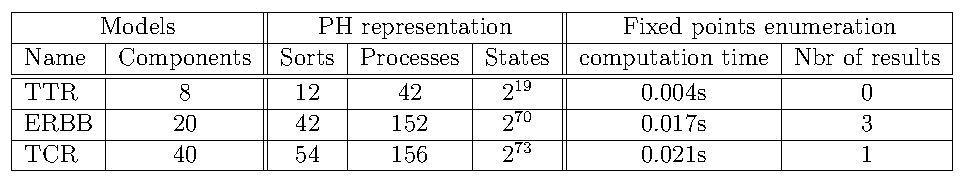
\includegraphics[width=\textwidth]{images/table1.pdf}
\caption{\label{tab:models}%
Description of the models used in our tests and results of our fixed point enumeration.
Each model is referred to by its short name, where
TTR stands for the tadpole tail resorption model% ~\cite{khalis2009smbionet},
ERBB for the receptor-regulated G1/S transition of the same name% ~\cite{Samaga2009}
and TCR for the T-cell receptor signaling network %\cite{Klamt06}.
For each of them, this table gives the number of biological components
in the original representation,
and the number of sorts, the number of processes
and the number of states in the PH model.
Finally, the last column gives the computation time for the enumeration of all fixed points
and the number of results returned.
}
\end{table}

\begin{table}[ht]
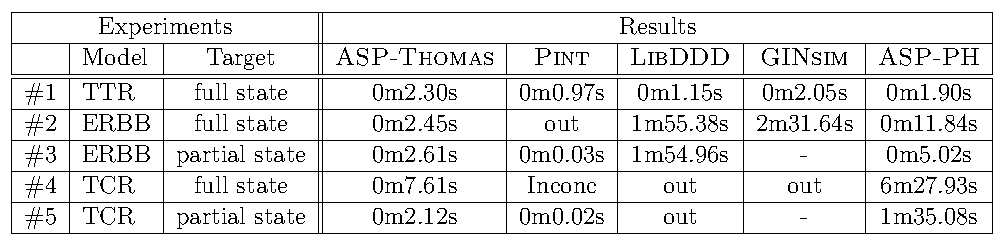
\includegraphics[width=\textwidth]{images/table2}
\caption{\label{tab:reachability}%
Compared performances of several methods to compute reachability analyses:
The method of Rocca \textit{et al.} (denoted by \textsc{ASP-Thomas}), \textsc{Pint}, \textsc{LibDDD}, \textsc{GINsim} and our new method presented in this paper, called \textsc{ASP-PH}.
For each test, this table gives the short name of the considered model,
as given in table~\ref{tab:models},
the type of goal (either a whole state or a sub-state)
and the computation time of the different methods used for the tests,
where “out” marks an execution taking too much time or memory,
\mbox{“~-~”} indicates that is not possible to do the test,
and “Inconc” states that the method terminates without a response.
}
\end{table}

\begin{itemize}

\item \textbf{ASP-Thomas}\footnote{These tests have been performed on another computer: dual core , 2.13 GHZ with 1.8 GB RAM. The authors wish to thank Laurent Trilling for his help.}
offers the possibility to model-check CTL properties of Thomas networks. 
There is no automatic way that allows the modelisation of Thomas networks in ASP. That is why it is necessary to study the entire network than to present it in ASP. But this modelisation takes so much time to be done regarding the complex representation of Thomas networks. Comparing with our method, we use the PH model which its actions are more easy to be presented in ASP, one fact per action.
In addition, the method "ASP-Thomas" requires to provide a maximum number of steps
for which the dynamics will be computed, which mays be difficult to be predicted.
However it is clear that this approach gives a very quick result when compared with others.
Indeed it also show that ASP is a good choice to run the dynamics of a model and check reachability properties. 
Furthermore, this method is able to check any kind of CTL formula
(and not only the “$\mathsf{EF}$” form that we focused on in this paper).
(see the discussion in section~\ref{limitations}).

\item \textbf{\textsc{GINsim}} is a software for the edition, simulation and analysis
of gene interaction networks.
It allows to compute all reachable stable states from a given initial state instantly;
however, it is not possible to compute all stable states independently from the initial state.
Regarding the reachability problem, \textsc{GINsim} only allows to check the reachability of
full states, because its approach consists in computing
all the state-transition graph and then search for a path between the two given states.
Therefore, it was not possible to perform reachability checks on partial states
(experiments \#3 \& \#5).
Small state-transition graphs can also be displayed by this tool.

\item \textbf{\textsc{LibDDD}}
is a library for symbolic model-checking of CTL \& LTL properties.
It can thus especially be used to check reachability properties;
however, as opposed to our method, it does not output an execution path
solving this reachability.
In addition, it relies on the construction of the state-transition graph
which is then stored under the form of a binary decision diagram for a more efficient analysis.
This computation explains why \textsc{LibDDD} takes more time to respond,
and gets out of memory in about 12 minutes for the biggest example
which contains $2^{73}$ states
(experiments \#4 \& \#5).
Finally, \textsc{LibDDD} is not able to compute the stable states of a network.

\item \textbf{\textsc{Pint}}
is a library gathering tools and converters related to the PH.
It should be noted that \textsc{Pint} contains the only reachability analysis
developed so far natively for the Process Hitting,
before the method proposed in this paper.
It consists in an approximation that avoids to compute the state-transition graph;
it is thus ensured to be really efficient, which explains the fastest results,
but at the cost of possibly terminating without being conclusive.
However, it is not designed for goals consisting of many processes,
which are more likely to trigger an inconclusive response
(such as for experiment \#4),
or an exponential research in sub-solutions
(such as for experiment \#2).
This explains the high computation times for some tests in table \ref{tab:reachability}.
Moreover, in the case of a positive answer,
it currently does not return the execution of the path achieving the desired reachability,
but only outputs its conclusion.
\end{itemize}

\subsection{Strengths and limitations of our method}
\label{limitations}

In the previous sections,
we developed new methods in ASP to check dynamical properties,
namely identifying stable states and finding all possible paths to reach a given goal.
Compared to some other methods describes above
(\textsc{GINsim}, \textsc{LibDDD} and the method \textsc{ASP-Thomas}) our method is relatively faster and also permits to study larger networks
(up to $2^{73}$ states in our tests). We study the networks which are modeled in Process Hitting. This new fomalisim for network modelisation is a restriction of synchronous automata so it allows to represent any kind of dynamical model. Moreover it is easy to implement the dynamics of the PH into ASP.
However, our ASP program may still be non-conclusive
in the cases where the given goal is not
reachable and the model contains loops in its dynamics
(which happens in almost every biological model).
In this case, the program will compute all infinite paths in these loops,
and never reach a goal or a fixed point.
It is still possible, however, to limit the number of iterations to an arbitrary
maximum which will be eventually reached in the case of an endless loop.
This is possible with the option \texttt{"-{}-imax=n"} of \textsc{iClingo},
where \texttt{n} is the maximum number of steps.
%%
%\begin{lstlisting}[numbers=none]
%iclingo find\_path.lp <network\_name>.lp -- imax=n
%\end{lstlisting}
%%

Several values can be given to this parameter.
For example, the total number of states is an obvious maximum,
as it will never be exceeded by a minimum path,
but it is too hight to be very interesting.
The total number of sorts is a more interesting value,
under the hypothesis that each one will change its active process at most once,
which is often the case for Boolean networks;
or, with a similar reasoning, the total number of processes can be chosen.
In these cases, however, a termination with no solution cannot be considered as a formal
negative answer, unless one can prove that the chosen value \texttt{n}
is bigger than the longest possible path in the state-transition graph.
Given our implementation, if the step \texttt{n} is reached,
the computation stops and there is no path to be displayed because there is no path which verifies the goals after \texttt{n} changes. Indeed this permits to get a final result, which is \texttt{unsatisfable} property after \texttt{n} steps so with this way we eliminate the unlimitaded execution time.


%\vspace{-1.0cm}

\section{Conclusion and future directions}
\label{sec:ccl}
In this paper, we gave a new method to compute some dynamical properties
on Process Hitting models, a subclass of asynchronous automata.
The main interest of our method is the use of ASP,
a declarative programming paradigm which benefits from powerful solvers.
We first focused on the enumeration of the fixed points of a model,
which is tackled simply on such models given their particular form.
We also considered the reachability problem, that is,
checking if it is possible to reach a state with a given property
from a given initial state,
which thus corresponds to an $\mathsf{EF}$ operator in CTL logic.
Our analysis is thus exhaustive, but can be limited to a number of steps,
for which the dynamics of the model from the given initial state is computed.
We gave an implementation of these problems into ASP,
and applied them to several biological examples of various sizes, up to
40 biological components.
Our results showed that our implementation is faster and deals with bigger models
than other approaches, especially \textsc{LibDDD} which is a symbolic model-checker.

Our work could benefit from several extensions.
Of course, the set of applicable models can be extended,
for example with the addition
of priorities or neutralizing edges,
or by considering synchronous dynamics or other representations
such as Thomas modeling~\cite{BernotSemBRN}.
However, the range of the analysis can also be extended,
by searching instead the set of initial states
allowing to reach a given goal,
or extending the method to universal properties (like the $\mathsf{AF}$ operator).
Finally, the research of attractors in a more general fashion
(such as cyclic or complex attractors)
would be of major interest to fully understand the behavior of models.

{\small
\paragraph{Acknowledgement}
The European Research Council has provided financial support
under the European Community's Seventh Framework Programme (FP7/2007--2013)~/
ERC grant agreement no.~259267.
}



%\clearpage
\bibliographystyle{acmtrans}
\bibliography{biblio}


\clearpage
\appendix

%\ssmall
In order to develop these methods we have used two main frameworks. The first is both a programming paradigm and a declarative programming language: the Answer Set Programming (ASP).
The second framework is the Process Hitting (PH) a previously introduced formalism for the representation of biological regulatory networks.

\subsection{Answer Set Programming }

\emph{Answer Set Programming} (ASP) is a declarative programming paradigm with semantics known as the \emph{semantics of answer sets}.
This paradigm allows the programmer to specify what the problem to be solved is, and not how to solve it.
ASP programs are written in AnsProlog* \cite{sureshkumar2006ansprolog} (short for “Answer Set Programming in Logic”).
These programs are composed of a set of \emph{facts} and a set of \emph{rules}, as defined below, from which other facts can be derived.
A consistent set of facts that can be derived from a program using the rules is called \emph{answer set} for the program.
The sets of possible responses to an AnsProlog* program are calculated with a program called a solver.

\subsubsection{Syntax and semantics of ASP}
\label{sectionSyntaxeASP}
\begin{enumerate}

\item \textbf{The alphabet}

According to \cite{baral2003knowledge}, the alphabet of ASP is composed of seven classes of symbols:
\begin{itemize}
  \item \emph{constants}, symbols of \emph{functions} and symbols of \emph{predicates} are composed of letters and start with a lowercase letter,
  \item \emph{variables} follow the same rule but start with a capital letter,
  \item \emph{connectors} that are “$\leftarrow$”, “$\textbf{not}$” and “$,$”,
  \item \emph{punctuation} that can be “(”, “)” and “.”,
  \item the special symbols “$\bot$” and “$\top$”.
\end{itemize}

The notion of predicate allows to qualify constants in this grammar.
For example, the property “\textit{Tweety is a bird}”
can be expressed by the predicate name \textit{bird}
around the constant \textit{tweety} into the following literal:
\textit{bird(tweety)}.
Such literal can then be used as premise or conclusion in a rule as defined below.

\item \textbf{The rules:}
A rule has the following form:
\begin{equation} \label{eq1ASP}
 head \leftarrow body.
\end{equation}
which is equivalent to:
\begin{equation} \label{eq2ASP}
l_{0} \leftarrow l_{1},...,l_{m}, \ASPnot l_{m+1},..., \ASPnot l_{n}.
\end{equation}
where $l_{i}$ are literals for all $i \in \llbracket 1 ; n \rrbracket$, and $0 \leq m \leq n$.
This rule states:
\[
\left.
    \begin{array}{rcl}
        \text{If } & l_{1},...,l_{m}  & \text{ \textbf{can} be proved true}\\
        \text{and } & l_{m+1},...,l_{n} & \text{ \textbf{cannot} be proved true}
    \end{array}
\right \} \text{Then} ~ l_{0} ~ \text{is } \textbf{true}.
\]

Therefore, “$head$” is also called the \emph{conclusion} of the rule,
and “$body$” is its \emph{premise}.
% An \emph{answer set} of a program (that is, a set of rules)
% is a minimal set of literals that satisfies all the rules.

There are some special cases of rules \cite{Vladimir,baral2003knowledge}:
\begin{itemize}
\item A \emph{ground} rule is a rule where all the literals are constants,
  and thus contains no variables;

\item A \emph{fact}, also called \emph{reality}, is a rule with an empty body.
  It can be written without the central arrow ($\leftarrow$) or with a $body$ equal to $\top$:
\begin{equation} 
l_{0} \leftarrow \top. \qquad \text{or} \qquad l_{0}.
 \label{eq5ASP}
\end{equation}

\item A \emph{constraint} is a rule where the head equals $\bot$.
  In this case, the head is often not represented and the constraint will be written generally as:
\begin{equation} 
  \leftarrow l_{1},...,l_{m}, \ASPnot l_{m+1},..., \ASPnot l_{n}.
  \label{eq6ASP}
\end{equation}
A set of literals $X$ \emph{violates} the constraint \eqref{eq6ASP} if $\{l_{1},...,l_{m}\} \subseteq X$ and $\{l_{m+1},...,l_{n}\} \nsubseteq X$.
Thus, $X$ cannot be an answer set of any program containing this constraint.
% If a program $\pi$ contains such a constraint $r$, then $X$ is an answer set of $\pi$ if and only if $X$ is an \textit{answer set} of $\pi \setminus \{r\}$ and $X$ does not violate $r$.

\item A \emph{cardinality constraint} is a rule of the following form:
\begin{equation} 
 ~ l ~\{q_{1},~ ... ,~ q_{m}\}~ u \leftarrow body.
 \label{eq7ASP}
\end{equation}
with $m \geq 1$, $l$ an integer and $u$ an integer or the infinity ($\infty$).
Such a cardinality means that the answer set $X$ contains
at least $l$ and at most $u$ atoms in the set $\{q_{1}, ... , q_{m}\}$,
or, in other words:
\begin{equation}
  l \leq | \{q_{1},... , q_{m}\} \cap X | \leq u
\end{equation}
where $\cap$ is the symbol of sets intersection
and $|A|$ denotes the cardinality of set $A$.
Thus, if such a cardinality is found in the head of a rule,
then it directly constrains the resulting answer set.
If it is found in the body of a rule,
then it is simply true if the above condition is satisfied.
In the following, if they are not explicitly given,
we consider that $l$ defaults to $0$ and $u$ defaults to $\infty$.

\end{itemize}


\end{enumerate}

\subsubsection{Modeling and solving of a problem with ASP}

The construction of models is one of the fundamental components of the scientific process.
It concerns all systems we seek to control.
A model has two main features \cite{Glimpse}:
it is a simplification of a given system
and it allows an action on the system like resolving problems, searching for a path, identifying states and verifying properties...
This concept of model can address another angle issues related to the representation process.
the programs written in ASP follow the strategy of “generate and test”.
Indeed, the modeling process can be regarded as a special form of representation:
\begin{itemize}
  \item First, the system should be presented with facts.
  \item Second, properties of the model can be explained with rules.
  \item Third, all candidate answers can be generated, usually using cardinalities.
  \item Finally, constraints allow to filter the answers and only the sets of predicates satisfying all these conditions will be returned which and considered as \emph{answer sets}.
\end{itemize}

Therefore, in practice, the solving of ASP programs relies on a \emph{grounder} and a \emph{solver}
that usually work together:
first the grounder is used to remove variables in order to achieve an equivalent but constant program,
then the solver computes all answer sets for this stabilized program~\cite{Vladimir,AnsPrologAPE}.
Amongst all available grounders for ASP, we can name
\textsc{Gringo}, \textsc{DLV} and \textsc{LParse},
and the solvers include
\textsc{SModels}, \textsc{DLV}, \textsc{CModels}, \textsc{Clasp}...

For the work presented in this paper, we worked with \textsc{Clingo} (version 3) which is a combination of the grounder \textsc{Gringo} and the solver \textsc{Clasp}.



\end{document}
